\documentclass{beamer}
\usefonttheme[onlymath]{serif}
\usepackage[english]{babel}							%For internationalization
\usepackage[utf8]{inputenc}							%For character encoding
\usepackage{amsmath}								%For mathematical typesetting
\usepackage{amssymb}								%For mathematical typesetting
\usepackage{graphicx}								%For handling graphics
\usepackage{listings}

\newcommand{\be}{\begin{equation}}
\newcommand{\bea}{\begin{equation*}}
\newcommand{\ben}[1]{\begin{equation}\label{#1}}
\newcommand{\ee}{\end{equation}}
\newcommand{\eea}{\end{equation*}}
\newcommand{\aq}{\overset{\sim}{q}}

\title
{An Introduction to Discontinuous Galerkin Methods}
\subtitle{Module 3A: To Higher-Orders - Solution Approximation}
\author[Bevan] % (optional, for multiple authors)
{J.~Bevan}
\institute[UMass Lowell]
{
  Department of Mechanical Engineering, Grad Student\\
  University of Massachusetts at Lowell
}
\date[Fall 2014]
{}
\subject{Discontinuous Galerkin}

\begin{document}
\frame{\titlepage}
\frame{\frametitle{Module 3A: To Higher-Orders - Solution Approximation}\tableofcontents}

%NEW SECTION
\section{Weak Form- Revisited}
\subsection{Approximation Space} 
\frame{\frametitle{\textbf{\secname}: \subsecname}
\be \int_{\Omega} \frac{\partial q}{\partial t} \phi_j \,dx + \int_{\Omega} \frac{\partial f(q)}{\partial x} \phi_j \,dx = 0 \ee
\begin{itemize}
\item Let's revisit the weak form in greater detail, we glossed over some important details.
\item To get a flexible method, we'd like to be able to generate an arbitrary order solution approximation. How do we do this in code?
\item We glossed over the construction of the bases, we can think in terms of nodal or modal
\be \aq(x) = \sum_{i=0}^M a_i \psi_i(x) \ee
\end{itemize}
}

\subsection{$L^2$ Projection: Minimize norm} 
\frame{\frametitle{\subsecname}
\begin{itemize}
\item Where does the weak form come from? Approximate sol'n doesn't satisfy the PDE exactly, left with some residual
\be \frac{\partial \aq}{\partial t} \,dx + \frac{\partial f(\aq)}{\partial x}\,dx = R(x) \ee
\item A projection finds the "closest" fit on a vector space compared to the original. An orthogonal projection does just this.
\item Minimizes the $L^2$ norm wrt the space projected upon
\end{itemize}
}

\subsection{The Galerkin Condition} 
\frame{\frametitle{\subsecname}
\begin{itemize}
\item An orthogonal projection means that the difference between the original and the projection should be orthogonal to the space projected upon, so for each basis $\phi \in V_h$
\be \int (f-f_h) \, \phi \,dx =0 = \int R(x) \phi \,dx\ee
\item The projected space doesn't have to be the same space as the solution approximation, but if we do choose them to be the same we have the Bubnov-Galerkin approach
\item We could choose the two spaces to be different, this is a Petrov-Galerkin approach. As an example, a weight space of delta functions yields a collocation method
\end{itemize}
}

%NEW SECTION
\section{Arbitrary Order Basis: Monomials?} 
\frame{\frametitle{\textbf{\secname}}
\begin{itemize}
\item Let's continue with the choice of polynomials for our basis functions.
\item The easy and obvious choice is the monomials $\psi_i(x) = a_i x^i$ so the arbitrary order solution approximation is
\be \aq(x) = \sum_{i=0}^M a_i \psi_i(x)= \sum_{i=0}^M a_i x^i  \ee
\item Can you think of why this a poor choice for a vector basis? Remember a basis needs to be complete and linearly independent. Let's see two separate ways why this is a poor choice.
\end{itemize}
}

\subsection{Linear Dependence} 
\frame{\frametitle{\subsecname}
\begin{itemize}
\item Normalize the basis wrt to the $L^2$ norm $\vert g \vert = \sqrt{\int g^2}$ so $\bar{\psi}_i=\sqrt{2i+1}x^i$ 
\item Consider the inner product of two adjacent basis functions
\be \int \bar{\psi}_{i-1} \bar{\psi}_{i} \,dx = \sqrt{1-\frac{1}{4i^2}} \ee
\item Linearly independent vectors are orthogonal, that is their inner product is zero. But for our monomials, even moderate values of $i$ give an inner product of close to 1
\item Very nearly dependent basis vectors mean small perturbations can lead to trouble finding the correct solution
\end{itemize}
}

\subsection{The ill-conditioned Hilbert matrix} 
\frame{\frametitle{\subsecname}
\begin{itemize}
\item The alternate way to consider this is to look at the mass matrix for a monomial basis
\item $1$
\item $x$
\item $x^2$
\item $x^3$
\item When we integrate from 0 to 1 it is easy to see the pattern of values, this is a Hilbert matrix
\item It is ill-conditioned, let's see why this is a problem in Matlab
\end{itemize}
}

%NEW SECTION
\section{[Recall] Lagrange Interpolation} 
\frame{\frametitle{\textbf{\secname}}
\begin{itemize}
\item Instead of a monomial basis, what if we were to use a Lagrange basis (commonly used for interpolation)
\item Recall, the Lagrange basis is zero at all interp nodes except the basis node, which it is 1 at
\item It has the form
\be L_q(x) = \prod_{p=1,p\neq q}^{Np} \frac{x-x_p}{x_q-x_p} \ee
\item We can compactly represent this as
nn=elim(nd(1:N)',nd(1:N)',[1 3 2]);\\
Lag= @(x,nv) prod(bsxfun(@rdivide,bsxfun(@minus,x,nn(nv,:,:)),...\\
bsxfun(@minus,nd(nv),nn(nv,:,:))),3);
\end{itemize}
}

%NEW SECTION
\section{Lagrange Spatial Approximation} 
\frame{\frametitle{\textbf{\secname}}
\begin{itemize}
\item We can now represent our arbitrary order sol'n approximation
\be \aq(x) = \sum_{i=0}^M a_i \psi_i(x)= \sum_{i=0}^M q(x_i) L_i(x)  \ee
\item Where we must choose a collection of points to use as our interpolation nodes
\end{itemize}
}

%NEW SECTION
\section{Interpolation Points: Equispaced?} 
\frame{\frametitle{\textbf{\secname}}
\begin{itemize}
\item It would seem logical that equispaced points are a good choice. They evenly cover the domain and are simple to calculate positions for.
\item Indeed these points work well for low $Np$, so one would expect the accuracy to increase as $Np$ increases
\item Let's see how it behaves at large $Np$
\end{itemize}
}

%NEW SECTION
\section{Runge's Phenomenon} 
\frame{\frametitle{\textbf{\secname}}
\begin{itemize}
\item The divergence of the interpolation is a result of Runge's phenomenon
\item Why this fails is explainable in terms of two relations: the Bernstein and Markov Inequalities. For a polynomial $P^N \in [-1, 1]$
\be |P^{\prime}(x)| \leq \frac{N}{\sqrt{1-x^2}}\| P \| _{\infty} \ee
\item The singularity in the Bernstein inequality can be bounded by the Markov inequality
\be \| P^{\prime} \| {\infty} \leq N^2 \| P \|_ {\infty} \ee
\item With the overall being
\be |P^{\prime}(x)| \leq \min \left(\frac{N}{\sqrt{1-x^2}},N^2\right)\| P \|_ {\infty} \ee

\end{itemize}
}

%NEW SECTION
\section{Interpolation Points: Legendre Roots} 
\frame{\frametitle{\textbf{\secname}}
\begin{itemize}
\item The overall inequality implies we'd like quadratic spacing near the element boundaries.
\item Though it may seem arbitrary, the roots of the Legendre polynomials have a favorable spacing that matches out needs
\item They avoid Runge's phenomenon, and have several other very nice features we shall see in the next module
\begin{figure}
\centering
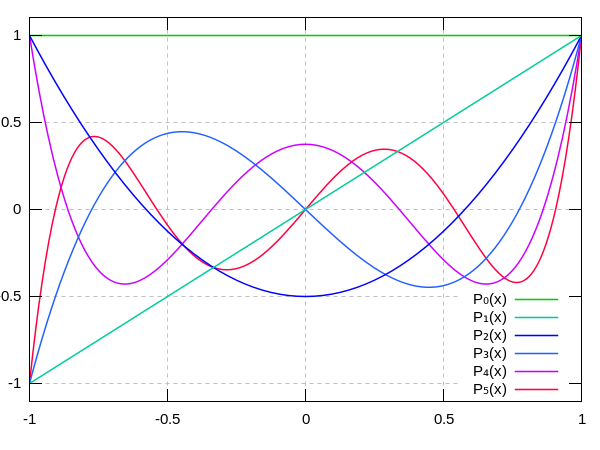
\includegraphics[width=2in]{LegPolys.PNG}
\end{figure}
\centering
\tiny http://en.wikipedia.org/wiki/File:Legendrepolynomials6.svg
\end{itemize}
}

\end{document}